\documentclass{article}
\usepackage{graphicx} % Required for inserting images
\usepackage{mwe} % for blindtext and example-image-a in example
\usepackage{wrapfig}
\usepackage[most]{tcolorbox}
\usepackage{float}
\usepackage[a4paper, total={7in, 9in}]{geometry}
\usepackage[framemethod=tikz]{mdframed}
\usepackage{hyperref}
\usepackage{amsthm}
\newtheorem{lemma}{Lemma}
\newtheorem{theorem}{Theorem}
\usepackage{listings}
\usepackage{cleveref}
\usepackage[most]{tcolorbox}
\usepackage{tikz}
\usepackage{color}
\usepackage{xcolor}
\usepackage{framed}
\usepackage{amsfonts}

\definecolor{light}{HTML}{c48fcd}
\definecolor{medium}{HTML}{a757b2}
\definecolor{dark}{HTML}{9637a0}
\definecolor{mygray}{gray}{0.95}
\definecolor{mypink}{rgb}{0.91, 0.98, 0.99}
\newcounter{problemnumber}
\setcounter{problemnumber}{0}
\usepackage{tgpagella}

\newenvironment{problem}[2]{
\addtocounter{problemnumber}{1}
\noindent
\begin{tikzpicture}
\draw[solid] (-8,-2) -- (8,-2);
\node (B) [fill=white,draw] at (2,-2)  {\textbf{Problem \theproblemnumber\  (#2)}};
\end{tikzpicture}
\newline
\begin{minipage}[t]{0.3\linewidth}
\raisebox{\dimexpr-\height+\ht\strutbox\relax}{\includegraphics[width=.88\textwidth]{#1}}
\end{minipage}
\hspace{.1mm}
\begin{minipage}[t]{0.7\linewidth}
}{
\end{minipage}
\color{white}.\color{black}\\[0cm]
\begin{tikzpicture}
\draw[solid] (-8,-2) -- (8,-2);
\end{tikzpicture}
\color{white}.\color{black}\\[1cm]
}

\newenvironment{hint}[1][\hsize]
{%
	\noindent
	
\begin{tikzpicture}
	\node (B) [fill=white,draw] at (2,-2)  {\textbf{Hint}};
	\end{tikzpicture}
	.\\[-0.8cm]
	\def\FrameCommand
	{%
		{\color{pink}\vrule width 3pt}%
		\hspace{0pt}%must no space.
		\fboxsep=\FrameSep\colorbox{mypink}%
	}%
	\MakeFramed{\hsize#1\advance\hsize-\width\FrameRestore}%
	\noindent
}
{\endMakeFramed}

\newenvironment{solution}[1][\hsize]
{%
	\noindent
	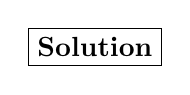
\begin{tikzpicture}
	\node (B) [fill=white,draw] at (2,-2)  {\textbf{Solution}};
	\end{tikzpicture}
	.\\[-0.8cm]
	\def\FrameCommand
	{%
		{\color{purple}\vrule width 3pt}%
		\hspace{0pt}%must no space.
		\fboxsep=\FrameSep\colorbox{mygray}%
	}%
	\MakeFramed{\hsize#1\advance\hsize-\width\FrameRestore}%
	\noindent
}
{\endMakeFramed}





\title{Math Cafe}

\begin{document}

%\begin{comment}
\begin{problem}{42/figs/pic.jpg}{Dragons on the Chess Board}Dragon is a special chess piece that can move to the cells specified in the picture.

How many ways can 3 dragon pieces be placed on an $8\times8$ chessboard in a way that no two can move to each other's places in one step.

\begin{center}
	\includegraphics[width=9cm]{42/figs/42_dragon.png}
\end{center}


Link to the problem on Twitter:  \url{https://twitter.com/Riazi_Cafe/status/1706574099131302222}\end{problem}
\begin{hint}.
	First, try to solve the following easier problem: Assume that we know that the starting position of a the dragon is a box whose index is odd. In this case, is there a way to kill the dragon? Is there a way to generalize this idea?
\end{hint}
\begin{solution}
	Consider the interval from floor 9 up to floor 15, and then down to floor 13. If an elevator is at a random point in this interval, when it reaches floor 13 It will go either up or down with equal probabilities.
	
	If an elevator is in this interval, it will definitely reach floor 13 sooner than any elevator outside this interval, and thus we can ignore elevators outside of this interval. If there are no elevators in this interval, the first elevator that reaches floor 13 will be going up.
	
	The probability that at least one elevator is in this interval is equal to 
	$1-(22/30)^2$.
	Moreover, due to symmetry, the first elevator from this interval that reaches floor 13 is 50\% likely to be going down. Therefore the answer is equal to:
	$\frac{1-(22/30)^2}{2} = 5/225.$
\end{solution}
\newpage

\begin{problem}{42/figs/pic.jpg}{Dragons on the Chess Board}Dragon is a special chess piece that can move to the cells specified in the picture.

How many ways can 3 dragon pieces be placed on an $8\times8$ chessboard in a way that no two can move to each other's places in one step.

\begin{center}
	\includegraphics[width=9cm]{42/figs/42_dragon.png}
\end{center}


Link to the problem on Twitter:  \url{https://twitter.com/Riazi_Cafe/status/1706574099131302222}\end{problem}
\begin{solution}
	Consider the interval from floor 9 up to floor 15, and then down to floor 13. If an elevator is at a random point in this interval, when it reaches floor 13 It will go either up or down with equal probabilities.
	
	If an elevator is in this interval, it will definitely reach floor 13 sooner than any elevator outside this interval, and thus we can ignore elevators outside of this interval. If there are no elevators in this interval, the first elevator that reaches floor 13 will be going up.
	
	The probability that at least one elevator is in this interval is equal to 
	$1-(22/30)^2$.
	Moreover, due to symmetry, the first elevator from this interval that reaches floor 13 is 50\% likely to be going down. Therefore the answer is equal to:
	$\frac{1-(22/30)^2}{2} = 5/225.$
\end{solution}
\newpage

\begin{problem}{42/figs/pic.jpg}{Dragons on the Chess Board}Dragon is a special chess piece that can move to the cells specified in the picture.

How many ways can 3 dragon pieces be placed on an $8\times8$ chessboard in a way that no two can move to each other's places in one step.

\begin{center}
	\includegraphics[width=9cm]{42/figs/42_dragon.png}
\end{center}


Link to the problem on Twitter:  \url{https://twitter.com/Riazi_Cafe/status/1706574099131302222}\end{problem}
\begin{solution}
	Consider the interval from floor 9 up to floor 15, and then down to floor 13. If an elevator is at a random point in this interval, when it reaches floor 13 It will go either up or down with equal probabilities.
	
	If an elevator is in this interval, it will definitely reach floor 13 sooner than any elevator outside this interval, and thus we can ignore elevators outside of this interval. If there are no elevators in this interval, the first elevator that reaches floor 13 will be going up.
	
	The probability that at least one elevator is in this interval is equal to 
	$1-(22/30)^2$.
	Moreover, due to symmetry, the first elevator from this interval that reaches floor 13 is 50\% likely to be going down. Therefore the answer is equal to:
	$\frac{1-(22/30)^2}{2} = 5/225.$
\end{solution}
\newpage

\begin{problem}{42/figs/pic.jpg}{Dragons on the Chess Board}Dragon is a special chess piece that can move to the cells specified in the picture.

How many ways can 3 dragon pieces be placed on an $8\times8$ chessboard in a way that no two can move to each other's places in one step.

\begin{center}
	\includegraphics[width=9cm]{42/figs/42_dragon.png}
\end{center}


Link to the problem on Twitter:  \url{https://twitter.com/Riazi_Cafe/status/1706574099131302222}\end{problem}
\begin{solution}
	Consider the interval from floor 9 up to floor 15, and then down to floor 13. If an elevator is at a random point in this interval, when it reaches floor 13 It will go either up or down with equal probabilities.
	
	If an elevator is in this interval, it will definitely reach floor 13 sooner than any elevator outside this interval, and thus we can ignore elevators outside of this interval. If there are no elevators in this interval, the first elevator that reaches floor 13 will be going up.
	
	The probability that at least one elevator is in this interval is equal to 
	$1-(22/30)^2$.
	Moreover, due to symmetry, the first elevator from this interval that reaches floor 13 is 50\% likely to be going down. Therefore the answer is equal to:
	$\frac{1-(22/30)^2}{2} = 5/225.$
\end{solution}
\newpage

\begin{problem}{42/figs/pic.jpg}{Dragons on the Chess Board}Dragon is a special chess piece that can move to the cells specified in the picture.

How many ways can 3 dragon pieces be placed on an $8\times8$ chessboard in a way that no two can move to each other's places in one step.

\begin{center}
	\includegraphics[width=9cm]{42/figs/42_dragon.png}
\end{center}


Link to the problem on Twitter:  \url{https://twitter.com/Riazi_Cafe/status/1706574099131302222}\end{problem}
\begin{solution}
	Consider the interval from floor 9 up to floor 15, and then down to floor 13. If an elevator is at a random point in this interval, when it reaches floor 13 It will go either up or down with equal probabilities.
	
	If an elevator is in this interval, it will definitely reach floor 13 sooner than any elevator outside this interval, and thus we can ignore elevators outside of this interval. If there are no elevators in this interval, the first elevator that reaches floor 13 will be going up.
	
	The probability that at least one elevator is in this interval is equal to 
	$1-(22/30)^2$.
	Moreover, due to symmetry, the first elevator from this interval that reaches floor 13 is 50\% likely to be going down. Therefore the answer is equal to:
	$\frac{1-(22/30)^2}{2} = 5/225.$
\end{solution}
\newpage

\begin{problem}{42/figs/pic.jpg}{Dragons on the Chess Board}Dragon is a special chess piece that can move to the cells specified in the picture.

How many ways can 3 dragon pieces be placed on an $8\times8$ chessboard in a way that no two can move to each other's places in one step.

\begin{center}
	\includegraphics[width=9cm]{42/figs/42_dragon.png}
\end{center}


Link to the problem on Twitter:  \url{https://twitter.com/Riazi_Cafe/status/1706574099131302222}\end{problem}
\begin{solution}
	Consider the interval from floor 9 up to floor 15, and then down to floor 13. If an elevator is at a random point in this interval, when it reaches floor 13 It will go either up or down with equal probabilities.
	
	If an elevator is in this interval, it will definitely reach floor 13 sooner than any elevator outside this interval, and thus we can ignore elevators outside of this interval. If there are no elevators in this interval, the first elevator that reaches floor 13 will be going up.
	
	The probability that at least one elevator is in this interval is equal to 
	$1-(22/30)^2$.
	Moreover, due to symmetry, the first elevator from this interval that reaches floor 13 is 50\% likely to be going down. Therefore the answer is equal to:
	$\frac{1-(22/30)^2}{2} = 5/225.$
\end{solution}
\newpage


\begin{problem}{42/figs/pic.jpg}{Dragons on the Chess Board}Dragon is a special chess piece that can move to the cells specified in the picture.

How many ways can 3 dragon pieces be placed on an $8\times8$ chessboard in a way that no two can move to each other's places in one step.

\begin{center}
	\includegraphics[width=9cm]{42/figs/42_dragon.png}
\end{center}


Link to the problem on Twitter:  \url{https://twitter.com/Riazi_Cafe/status/1706574099131302222}\end{problem}
\begin{solution}
	Consider the interval from floor 9 up to floor 15, and then down to floor 13. If an elevator is at a random point in this interval, when it reaches floor 13 It will go either up or down with equal probabilities.
	
	If an elevator is in this interval, it will definitely reach floor 13 sooner than any elevator outside this interval, and thus we can ignore elevators outside of this interval. If there are no elevators in this interval, the first elevator that reaches floor 13 will be going up.
	
	The probability that at least one elevator is in this interval is equal to 
	$1-(22/30)^2$.
	Moreover, due to symmetry, the first elevator from this interval that reaches floor 13 is 50\% likely to be going down. Therefore the answer is equal to:
	$\frac{1-(22/30)^2}{2} = 5/225.$
\end{solution}
\newpage


\begin{problem}{42/figs/pic.jpg}{Dragons on the Chess Board}Dragon is a special chess piece that can move to the cells specified in the picture.

How many ways can 3 dragon pieces be placed on an $8\times8$ chessboard in a way that no two can move to each other's places in one step.

\begin{center}
	\includegraphics[width=9cm]{42/figs/42_dragon.png}
\end{center}


Link to the problem on Twitter:  \url{https://twitter.com/Riazi_Cafe/status/1706574099131302222}\end{problem}
\begin{solution}
	Consider the interval from floor 9 up to floor 15, and then down to floor 13. If an elevator is at a random point in this interval, when it reaches floor 13 It will go either up or down with equal probabilities.
	
	If an elevator is in this interval, it will definitely reach floor 13 sooner than any elevator outside this interval, and thus we can ignore elevators outside of this interval. If there are no elevators in this interval, the first elevator that reaches floor 13 will be going up.
	
	The probability that at least one elevator is in this interval is equal to 
	$1-(22/30)^2$.
	Moreover, due to symmetry, the first elevator from this interval that reaches floor 13 is 50\% likely to be going down. Therefore the answer is equal to:
	$\frac{1-(22/30)^2}{2} = 5/225.$
\end{solution}
\newpage


\begin{problem}{42/figs/pic.jpg}{Dragons on the Chess Board}Dragon is a special chess piece that can move to the cells specified in the picture.

How many ways can 3 dragon pieces be placed on an $8\times8$ chessboard in a way that no two can move to each other's places in one step.

\begin{center}
	\includegraphics[width=9cm]{42/figs/42_dragon.png}
\end{center}


Link to the problem on Twitter:  \url{https://twitter.com/Riazi_Cafe/status/1706574099131302222}\end{problem}
\begin{solution}
	Consider the interval from floor 9 up to floor 15, and then down to floor 13. If an elevator is at a random point in this interval, when it reaches floor 13 It will go either up or down with equal probabilities.
	
	If an elevator is in this interval, it will definitely reach floor 13 sooner than any elevator outside this interval, and thus we can ignore elevators outside of this interval. If there are no elevators in this interval, the first elevator that reaches floor 13 will be going up.
	
	The probability that at least one elevator is in this interval is equal to 
	$1-(22/30)^2$.
	Moreover, due to symmetry, the first elevator from this interval that reaches floor 13 is 50\% likely to be going down. Therefore the answer is equal to:
	$\frac{1-(22/30)^2}{2} = 5/225.$
\end{solution}
\newpage

\begin{problem}{42/figs/pic.jpg}{Dragons on the Chess Board}Dragon is a special chess piece that can move to the cells specified in the picture.

How many ways can 3 dragon pieces be placed on an $8\times8$ chessboard in a way that no two can move to each other's places in one step.

\begin{center}
	\includegraphics[width=9cm]{42/figs/42_dragon.png}
\end{center}


Link to the problem on Twitter:  \url{https://twitter.com/Riazi_Cafe/status/1706574099131302222}\end{problem}
\begin{solution}
	Consider the interval from floor 9 up to floor 15, and then down to floor 13. If an elevator is at a random point in this interval, when it reaches floor 13 It will go either up or down with equal probabilities.
	
	If an elevator is in this interval, it will definitely reach floor 13 sooner than any elevator outside this interval, and thus we can ignore elevators outside of this interval. If there are no elevators in this interval, the first elevator that reaches floor 13 will be going up.
	
	The probability that at least one elevator is in this interval is equal to 
	$1-(22/30)^2$.
	Moreover, due to symmetry, the first elevator from this interval that reaches floor 13 is 50\% likely to be going down. Therefore the answer is equal to:
	$\frac{1-(22/30)^2}{2} = 5/225.$
\end{solution}
\newpage


\begin{problem}{42/figs/pic.jpg}{Dragons on the Chess Board}Dragon is a special chess piece that can move to the cells specified in the picture.

How many ways can 3 dragon pieces be placed on an $8\times8$ chessboard in a way that no two can move to each other's places in one step.

\begin{center}
	\includegraphics[width=9cm]{42/figs/42_dragon.png}
\end{center}


Link to the problem on Twitter:  \url{https://twitter.com/Riazi_Cafe/status/1706574099131302222}\end{problem}
\begin{solution}
	Consider the interval from floor 9 up to floor 15, and then down to floor 13. If an elevator is at a random point in this interval, when it reaches floor 13 It will go either up or down with equal probabilities.
	
	If an elevator is in this interval, it will definitely reach floor 13 sooner than any elevator outside this interval, and thus we can ignore elevators outside of this interval. If there are no elevators in this interval, the first elevator that reaches floor 13 will be going up.
	
	The probability that at least one elevator is in this interval is equal to 
	$1-(22/30)^2$.
	Moreover, due to symmetry, the first elevator from this interval that reaches floor 13 is 50\% likely to be going down. Therefore the answer is equal to:
	$\frac{1-(22/30)^2}{2} = 5/225.$
\end{solution}
\newpage


\begin{problem}{42/figs/pic.jpg}{Dragons on the Chess Board}Dragon is a special chess piece that can move to the cells specified in the picture.

How many ways can 3 dragon pieces be placed on an $8\times8$ chessboard in a way that no two can move to each other's places in one step.

\begin{center}
	\includegraphics[width=9cm]{42/figs/42_dragon.png}
\end{center}


Link to the problem on Twitter:  \url{https://twitter.com/Riazi_Cafe/status/1706574099131302222}\end{problem}
\begin{solution}
	Consider the interval from floor 9 up to floor 15, and then down to floor 13. If an elevator is at a random point in this interval, when it reaches floor 13 It will go either up or down with equal probabilities.
	
	If an elevator is in this interval, it will definitely reach floor 13 sooner than any elevator outside this interval, and thus we can ignore elevators outside of this interval. If there are no elevators in this interval, the first elevator that reaches floor 13 will be going up.
	
	The probability that at least one elevator is in this interval is equal to 
	$1-(22/30)^2$.
	Moreover, due to symmetry, the first elevator from this interval that reaches floor 13 is 50\% likely to be going down. Therefore the answer is equal to:
	$\frac{1-(22/30)^2}{2} = 5/225.$
\end{solution}
\newpage


\begin{problem}{42/figs/pic.jpg}{Dragons on the Chess Board}Dragon is a special chess piece that can move to the cells specified in the picture.

How many ways can 3 dragon pieces be placed on an $8\times8$ chessboard in a way that no two can move to each other's places in one step.

\begin{center}
	\includegraphics[width=9cm]{42/figs/42_dragon.png}
\end{center}


Link to the problem on Twitter:  \url{https://twitter.com/Riazi_Cafe/status/1706574099131302222}\end{problem}
\begin{solution}
	Consider the interval from floor 9 up to floor 15, and then down to floor 13. If an elevator is at a random point in this interval, when it reaches floor 13 It will go either up or down with equal probabilities.
	
	If an elevator is in this interval, it will definitely reach floor 13 sooner than any elevator outside this interval, and thus we can ignore elevators outside of this interval. If there are no elevators in this interval, the first elevator that reaches floor 13 will be going up.
	
	The probability that at least one elevator is in this interval is equal to 
	$1-(22/30)^2$.
	Moreover, due to symmetry, the first elevator from this interval that reaches floor 13 is 50\% likely to be going down. Therefore the answer is equal to:
	$\frac{1-(22/30)^2}{2} = 5/225.$
\end{solution}
\newpage


\begin{problem}{42/figs/pic.jpg}{Dragons on the Chess Board}Dragon is a special chess piece that can move to the cells specified in the picture.

How many ways can 3 dragon pieces be placed on an $8\times8$ chessboard in a way that no two can move to each other's places in one step.

\begin{center}
	\includegraphics[width=9cm]{42/figs/42_dragon.png}
\end{center}


Link to the problem on Twitter:  \url{https://twitter.com/Riazi_Cafe/status/1706574099131302222}\end{problem}
\begin{solution}
	Consider the interval from floor 9 up to floor 15, and then down to floor 13. If an elevator is at a random point in this interval, when it reaches floor 13 It will go either up or down with equal probabilities.
	
	If an elevator is in this interval, it will definitely reach floor 13 sooner than any elevator outside this interval, and thus we can ignore elevators outside of this interval. If there are no elevators in this interval, the first elevator that reaches floor 13 will be going up.
	
	The probability that at least one elevator is in this interval is equal to 
	$1-(22/30)^2$.
	Moreover, due to symmetry, the first elevator from this interval that reaches floor 13 is 50\% likely to be going down. Therefore the answer is equal to:
	$\frac{1-(22/30)^2}{2} = 5/225.$
\end{solution}
\newpage


\begin{problem}{42/figs/pic.jpg}{Dragons on the Chess Board}Dragon is a special chess piece that can move to the cells specified in the picture.

How many ways can 3 dragon pieces be placed on an $8\times8$ chessboard in a way that no two can move to each other's places in one step.

\begin{center}
	\includegraphics[width=9cm]{42/figs/42_dragon.png}
\end{center}


Link to the problem on Twitter:  \url{https://twitter.com/Riazi_Cafe/status/1706574099131302222}\end{problem}
\begin{solution}
	Consider the interval from floor 9 up to floor 15, and then down to floor 13. If an elevator is at a random point in this interval, when it reaches floor 13 It will go either up or down with equal probabilities.
	
	If an elevator is in this interval, it will definitely reach floor 13 sooner than any elevator outside this interval, and thus we can ignore elevators outside of this interval. If there are no elevators in this interval, the first elevator that reaches floor 13 will be going up.
	
	The probability that at least one elevator is in this interval is equal to 
	$1-(22/30)^2$.
	Moreover, due to symmetry, the first elevator from this interval that reaches floor 13 is 50\% likely to be going down. Therefore the answer is equal to:
	$\frac{1-(22/30)^2}{2} = 5/225.$
\end{solution}
\newpage



\begin{problem}{42/figs/pic.jpg}{Dragons on the Chess Board}Dragon is a special chess piece that can move to the cells specified in the picture.

How many ways can 3 dragon pieces be placed on an $8\times8$ chessboard in a way that no two can move to each other's places in one step.

\begin{center}
	\includegraphics[width=9cm]{42/figs/42_dragon.png}
\end{center}


Link to the problem on Twitter:  \url{https://twitter.com/Riazi_Cafe/status/1706574099131302222}\end{problem}
\begin{solution}
	Consider the interval from floor 9 up to floor 15, and then down to floor 13. If an elevator is at a random point in this interval, when it reaches floor 13 It will go either up or down with equal probabilities.
	
	If an elevator is in this interval, it will definitely reach floor 13 sooner than any elevator outside this interval, and thus we can ignore elevators outside of this interval. If there are no elevators in this interval, the first elevator that reaches floor 13 will be going up.
	
	The probability that at least one elevator is in this interval is equal to 
	$1-(22/30)^2$.
	Moreover, due to symmetry, the first elevator from this interval that reaches floor 13 is 50\% likely to be going down. Therefore the answer is equal to:
	$\frac{1-(22/30)^2}{2} = 5/225.$
\end{solution}
\newpage


\begin{problem}{42/figs/pic.jpg}{Dragons on the Chess Board}Dragon is a special chess piece that can move to the cells specified in the picture.

How many ways can 3 dragon pieces be placed on an $8\times8$ chessboard in a way that no two can move to each other's places in one step.

\begin{center}
	\includegraphics[width=9cm]{42/figs/42_dragon.png}
\end{center}


Link to the problem on Twitter:  \url{https://twitter.com/Riazi_Cafe/status/1706574099131302222}\end{problem}
\begin{hint}.
	First, try to solve the following easier problem: Assume that we know that the starting position of a the dragon is a box whose index is odd. In this case, is there a way to kill the dragon? Is there a way to generalize this idea?
\end{hint}
\begin{solution}
	Consider the interval from floor 9 up to floor 15, and then down to floor 13. If an elevator is at a random point in this interval, when it reaches floor 13 It will go either up or down with equal probabilities.
	
	If an elevator is in this interval, it will definitely reach floor 13 sooner than any elevator outside this interval, and thus we can ignore elevators outside of this interval. If there are no elevators in this interval, the first elevator that reaches floor 13 will be going up.
	
	The probability that at least one elevator is in this interval is equal to 
	$1-(22/30)^2$.
	Moreover, due to symmetry, the first elevator from this interval that reaches floor 13 is 50\% likely to be going down. Therefore the answer is equal to:
	$\frac{1-(22/30)^2}{2} = 5/225.$
\end{solution}
\newpage


\begin{problem}{42/figs/pic.jpg}{Dragons on the Chess Board}Dragon is a special chess piece that can move to the cells specified in the picture.

How many ways can 3 dragon pieces be placed on an $8\times8$ chessboard in a way that no two can move to each other's places in one step.

\begin{center}
	\includegraphics[width=9cm]{42/figs/42_dragon.png}
\end{center}


Link to the problem on Twitter:  \url{https://twitter.com/Riazi_Cafe/status/1706574099131302222}\end{problem}
\begin{solution}
	Consider the interval from floor 9 up to floor 15, and then down to floor 13. If an elevator is at a random point in this interval, when it reaches floor 13 It will go either up or down with equal probabilities.
	
	If an elevator is in this interval, it will definitely reach floor 13 sooner than any elevator outside this interval, and thus we can ignore elevators outside of this interval. If there are no elevators in this interval, the first elevator that reaches floor 13 will be going up.
	
	The probability that at least one elevator is in this interval is equal to 
	$1-(22/30)^2$.
	Moreover, due to symmetry, the first elevator from this interval that reaches floor 13 is 50\% likely to be going down. Therefore the answer is equal to:
	$\frac{1-(22/30)^2}{2} = 5/225.$
\end{solution}
\newpage


\begin{problem}{42/figs/pic.jpg}{Dragons on the Chess Board}Dragon is a special chess piece that can move to the cells specified in the picture.

How many ways can 3 dragon pieces be placed on an $8\times8$ chessboard in a way that no two can move to each other's places in one step.

\begin{center}
	\includegraphics[width=9cm]{42/figs/42_dragon.png}
\end{center}


Link to the problem on Twitter:  \url{https://twitter.com/Riazi_Cafe/status/1706574099131302222}\end{problem}
\begin{solution}
	Consider the interval from floor 9 up to floor 15, and then down to floor 13. If an elevator is at a random point in this interval, when it reaches floor 13 It will go either up or down with equal probabilities.
	
	If an elevator is in this interval, it will definitely reach floor 13 sooner than any elevator outside this interval, and thus we can ignore elevators outside of this interval. If there are no elevators in this interval, the first elevator that reaches floor 13 will be going up.
	
	The probability that at least one elevator is in this interval is equal to 
	$1-(22/30)^2$.
	Moreover, due to symmetry, the first elevator from this interval that reaches floor 13 is 50\% likely to be going down. Therefore the answer is equal to:
	$\frac{1-(22/30)^2}{2} = 5/225.$
\end{solution}
\newpage


\begin{problem}{42/figs/pic.jpg}{Dragons on the Chess Board}Dragon is a special chess piece that can move to the cells specified in the picture.

How many ways can 3 dragon pieces be placed on an $8\times8$ chessboard in a way that no two can move to each other's places in one step.

\begin{center}
	\includegraphics[width=9cm]{42/figs/42_dragon.png}
\end{center}


Link to the problem on Twitter:  \url{https://twitter.com/Riazi_Cafe/status/1706574099131302222}\end{problem}
\begin{solution}
	Consider the interval from floor 9 up to floor 15, and then down to floor 13. If an elevator is at a random point in this interval, when it reaches floor 13 It will go either up or down with equal probabilities.
	
	If an elevator is in this interval, it will definitely reach floor 13 sooner than any elevator outside this interval, and thus we can ignore elevators outside of this interval. If there are no elevators in this interval, the first elevator that reaches floor 13 will be going up.
	
	The probability that at least one elevator is in this interval is equal to 
	$1-(22/30)^2$.
	Moreover, due to symmetry, the first elevator from this interval that reaches floor 13 is 50\% likely to be going down. Therefore the answer is equal to:
	$\frac{1-(22/30)^2}{2} = 5/225.$
\end{solution}
\newpage


\begin{problem}{42/figs/pic.jpg}{Dragons on the Chess Board}Dragon is a special chess piece that can move to the cells specified in the picture.

How many ways can 3 dragon pieces be placed on an $8\times8$ chessboard in a way that no two can move to each other's places in one step.

\begin{center}
	\includegraphics[width=9cm]{42/figs/42_dragon.png}
\end{center}


Link to the problem on Twitter:  \url{https://twitter.com/Riazi_Cafe/status/1706574099131302222}\end{problem}
\begin{solution}
	Consider the interval from floor 9 up to floor 15, and then down to floor 13. If an elevator is at a random point in this interval, when it reaches floor 13 It will go either up or down with equal probabilities.
	
	If an elevator is in this interval, it will definitely reach floor 13 sooner than any elevator outside this interval, and thus we can ignore elevators outside of this interval. If there are no elevators in this interval, the first elevator that reaches floor 13 will be going up.
	
	The probability that at least one elevator is in this interval is equal to 
	$1-(22/30)^2$.
	Moreover, due to symmetry, the first elevator from this interval that reaches floor 13 is 50\% likely to be going down. Therefore the answer is equal to:
	$\frac{1-(22/30)^2}{2} = 5/225.$
\end{solution}
\newpage

\begin{problem}{42/figs/pic.jpg}{Dragons on the Chess Board}Dragon is a special chess piece that can move to the cells specified in the picture.

How many ways can 3 dragon pieces be placed on an $8\times8$ chessboard in a way that no two can move to each other's places in one step.

\begin{center}
	\includegraphics[width=9cm]{42/figs/42_dragon.png}
\end{center}


Link to the problem on Twitter:  \url{https://twitter.com/Riazi_Cafe/status/1706574099131302222}\end{problem}
\begin{solution}
	Consider the interval from floor 9 up to floor 15, and then down to floor 13. If an elevator is at a random point in this interval, when it reaches floor 13 It will go either up or down with equal probabilities.
	
	If an elevator is in this interval, it will definitely reach floor 13 sooner than any elevator outside this interval, and thus we can ignore elevators outside of this interval. If there are no elevators in this interval, the first elevator that reaches floor 13 will be going up.
	
	The probability that at least one elevator is in this interval is equal to 
	$1-(22/30)^2$.
	Moreover, due to symmetry, the first elevator from this interval that reaches floor 13 is 50\% likely to be going down. Therefore the answer is equal to:
	$\frac{1-(22/30)^2}{2} = 5/225.$
\end{solution}
\newpage

\begin{problem}{42/figs/pic.jpg}{Dragons on the Chess Board}Dragon is a special chess piece that can move to the cells specified in the picture.

How many ways can 3 dragon pieces be placed on an $8\times8$ chessboard in a way that no two can move to each other's places in one step.

\begin{center}
	\includegraphics[width=9cm]{42/figs/42_dragon.png}
\end{center}


Link to the problem on Twitter:  \url{https://twitter.com/Riazi_Cafe/status/1706574099131302222}\end{problem}
\begin{solution}
	Consider the interval from floor 9 up to floor 15, and then down to floor 13. If an elevator is at a random point in this interval, when it reaches floor 13 It will go either up or down with equal probabilities.
	
	If an elevator is in this interval, it will definitely reach floor 13 sooner than any elevator outside this interval, and thus we can ignore elevators outside of this interval. If there are no elevators in this interval, the first elevator that reaches floor 13 will be going up.
	
	The probability that at least one elevator is in this interval is equal to 
	$1-(22/30)^2$.
	Moreover, due to symmetry, the first elevator from this interval that reaches floor 13 is 50\% likely to be going down. Therefore the answer is equal to:
	$\frac{1-(22/30)^2}{2} = 5/225.$
\end{solution}
\newpage

\begin{problem}{42/figs/pic.jpg}{Dragons on the Chess Board}Dragon is a special chess piece that can move to the cells specified in the picture.

How many ways can 3 dragon pieces be placed on an $8\times8$ chessboard in a way that no two can move to each other's places in one step.

\begin{center}
	\includegraphics[width=9cm]{42/figs/42_dragon.png}
\end{center}


Link to the problem on Twitter:  \url{https://twitter.com/Riazi_Cafe/status/1706574099131302222}\end{problem}
\begin{solution}
	Consider the interval from floor 9 up to floor 15, and then down to floor 13. If an elevator is at a random point in this interval, when it reaches floor 13 It will go either up or down with equal probabilities.
	
	If an elevator is in this interval, it will definitely reach floor 13 sooner than any elevator outside this interval, and thus we can ignore elevators outside of this interval. If there are no elevators in this interval, the first elevator that reaches floor 13 will be going up.
	
	The probability that at least one elevator is in this interval is equal to 
	$1-(22/30)^2$.
	Moreover, due to symmetry, the first elevator from this interval that reaches floor 13 is 50\% likely to be going down. Therefore the answer is equal to:
	$\frac{1-(22/30)^2}{2} = 5/225.$
\end{solution}
\newpage



\begin{problem}{42/figs/pic.jpg}{Dragons on the Chess Board}Dragon is a special chess piece that can move to the cells specified in the picture.

How many ways can 3 dragon pieces be placed on an $8\times8$ chessboard in a way that no two can move to each other's places in one step.

\begin{center}
	\includegraphics[width=9cm]{42/figs/42_dragon.png}
\end{center}


Link to the problem on Twitter:  \url{https://twitter.com/Riazi_Cafe/status/1706574099131302222}\end{problem}
\begin{solution}
	Consider the interval from floor 9 up to floor 15, and then down to floor 13. If an elevator is at a random point in this interval, when it reaches floor 13 It will go either up or down with equal probabilities.
	
	If an elevator is in this interval, it will definitely reach floor 13 sooner than any elevator outside this interval, and thus we can ignore elevators outside of this interval. If there are no elevators in this interval, the first elevator that reaches floor 13 will be going up.
	
	The probability that at least one elevator is in this interval is equal to 
	$1-(22/30)^2$.
	Moreover, due to symmetry, the first elevator from this interval that reaches floor 13 is 50\% likely to be going down. Therefore the answer is equal to:
	$\frac{1-(22/30)^2}{2} = 5/225.$
\end{solution}
\newpage


\begin{problem}{42/figs/pic.jpg}{Dragons on the Chess Board}Dragon is a special chess piece that can move to the cells specified in the picture.

How many ways can 3 dragon pieces be placed on an $8\times8$ chessboard in a way that no two can move to each other's places in one step.

\begin{center}
	\includegraphics[width=9cm]{42/figs/42_dragon.png}
\end{center}


Link to the problem on Twitter:  \url{https://twitter.com/Riazi_Cafe/status/1706574099131302222}\end{problem}
\begin{solution}
	Consider the interval from floor 9 up to floor 15, and then down to floor 13. If an elevator is at a random point in this interval, when it reaches floor 13 It will go either up or down with equal probabilities.
	
	If an elevator is in this interval, it will definitely reach floor 13 sooner than any elevator outside this interval, and thus we can ignore elevators outside of this interval. If there are no elevators in this interval, the first elevator that reaches floor 13 will be going up.
	
	The probability that at least one elevator is in this interval is equal to 
	$1-(22/30)^2$.
	Moreover, due to symmetry, the first elevator from this interval that reaches floor 13 is 50\% likely to be going down. Therefore the answer is equal to:
	$\frac{1-(22/30)^2}{2} = 5/225.$
\end{solution}
\newpage


\begin{problem}{42/figs/pic.jpg}{Dragons on the Chess Board}Dragon is a special chess piece that can move to the cells specified in the picture.

How many ways can 3 dragon pieces be placed on an $8\times8$ chessboard in a way that no two can move to each other's places in one step.

\begin{center}
	\includegraphics[width=9cm]{42/figs/42_dragon.png}
\end{center}


Link to the problem on Twitter:  \url{https://twitter.com/Riazi_Cafe/status/1706574099131302222}\end{problem}
\begin{solution}
	Consider the interval from floor 9 up to floor 15, and then down to floor 13. If an elevator is at a random point in this interval, when it reaches floor 13 It will go either up or down with equal probabilities.
	
	If an elevator is in this interval, it will definitely reach floor 13 sooner than any elevator outside this interval, and thus we can ignore elevators outside of this interval. If there are no elevators in this interval, the first elevator that reaches floor 13 will be going up.
	
	The probability that at least one elevator is in this interval is equal to 
	$1-(22/30)^2$.
	Moreover, due to symmetry, the first elevator from this interval that reaches floor 13 is 50\% likely to be going down. Therefore the answer is equal to:
	$\frac{1-(22/30)^2}{2} = 5/225.$
\end{solution}
\newpage


\begin{problem}{42/figs/pic.jpg}{Dragons on the Chess Board}Dragon is a special chess piece that can move to the cells specified in the picture.

How many ways can 3 dragon pieces be placed on an $8\times8$ chessboard in a way that no two can move to each other's places in one step.

\begin{center}
	\includegraphics[width=9cm]{42/figs/42_dragon.png}
\end{center}


Link to the problem on Twitter:  \url{https://twitter.com/Riazi_Cafe/status/1706574099131302222}\end{problem}
\begin{solution}
	Consider the interval from floor 9 up to floor 15, and then down to floor 13. If an elevator is at a random point in this interval, when it reaches floor 13 It will go either up or down with equal probabilities.
	
	If an elevator is in this interval, it will definitely reach floor 13 sooner than any elevator outside this interval, and thus we can ignore elevators outside of this interval. If there are no elevators in this interval, the first elevator that reaches floor 13 will be going up.
	
	The probability that at least one elevator is in this interval is equal to 
	$1-(22/30)^2$.
	Moreover, due to symmetry, the first elevator from this interval that reaches floor 13 is 50\% likely to be going down. Therefore the answer is equal to:
	$\frac{1-(22/30)^2}{2} = 5/225.$
\end{solution}
\newpage


\begin{problem}{42/figs/pic.jpg}{Dragons on the Chess Board}Dragon is a special chess piece that can move to the cells specified in the picture.

How many ways can 3 dragon pieces be placed on an $8\times8$ chessboard in a way that no two can move to each other's places in one step.

\begin{center}
	\includegraphics[width=9cm]{42/figs/42_dragon.png}
\end{center}


Link to the problem on Twitter:  \url{https://twitter.com/Riazi_Cafe/status/1706574099131302222}\end{problem}
\begin{solution}
	Consider the interval from floor 9 up to floor 15, and then down to floor 13. If an elevator is at a random point in this interval, when it reaches floor 13 It will go either up or down with equal probabilities.
	
	If an elevator is in this interval, it will definitely reach floor 13 sooner than any elevator outside this interval, and thus we can ignore elevators outside of this interval. If there are no elevators in this interval, the first elevator that reaches floor 13 will be going up.
	
	The probability that at least one elevator is in this interval is equal to 
	$1-(22/30)^2$.
	Moreover, due to symmetry, the first elevator from this interval that reaches floor 13 is 50\% likely to be going down. Therefore the answer is equal to:
	$\frac{1-(22/30)^2}{2} = 5/225.$
\end{solution}
\newpage


\begin{problem}{42/figs/pic.jpg}{Dragons on the Chess Board}Dragon is a special chess piece that can move to the cells specified in the picture.

How many ways can 3 dragon pieces be placed on an $8\times8$ chessboard in a way that no two can move to each other's places in one step.

\begin{center}
	\includegraphics[width=9cm]{42/figs/42_dragon.png}
\end{center}


Link to the problem on Twitter:  \url{https://twitter.com/Riazi_Cafe/status/1706574099131302222}\end{problem}
\begin{solution}
	Consider the interval from floor 9 up to floor 15, and then down to floor 13. If an elevator is at a random point in this interval, when it reaches floor 13 It will go either up or down with equal probabilities.
	
	If an elevator is in this interval, it will definitely reach floor 13 sooner than any elevator outside this interval, and thus we can ignore elevators outside of this interval. If there are no elevators in this interval, the first elevator that reaches floor 13 will be going up.
	
	The probability that at least one elevator is in this interval is equal to 
	$1-(22/30)^2$.
	Moreover, due to symmetry, the first elevator from this interval that reaches floor 13 is 50\% likely to be going down. Therefore the answer is equal to:
	$\frac{1-(22/30)^2}{2} = 5/225.$
\end{solution}
\newpage


\begin{problem}{42/figs/pic.jpg}{Dragons on the Chess Board}Dragon is a special chess piece that can move to the cells specified in the picture.

How many ways can 3 dragon pieces be placed on an $8\times8$ chessboard in a way that no two can move to each other's places in one step.

\begin{center}
	\includegraphics[width=9cm]{42/figs/42_dragon.png}
\end{center}


Link to the problem on Twitter:  \url{https://twitter.com/Riazi_Cafe/status/1706574099131302222}\end{problem}
\begin{solution}
	Consider the interval from floor 9 up to floor 15, and then down to floor 13. If an elevator is at a random point in this interval, when it reaches floor 13 It will go either up or down with equal probabilities.
	
	If an elevator is in this interval, it will definitely reach floor 13 sooner than any elevator outside this interval, and thus we can ignore elevators outside of this interval. If there are no elevators in this interval, the first elevator that reaches floor 13 will be going up.
	
	The probability that at least one elevator is in this interval is equal to 
	$1-(22/30)^2$.
	Moreover, due to symmetry, the first elevator from this interval that reaches floor 13 is 50\% likely to be going down. Therefore the answer is equal to:
	$\frac{1-(22/30)^2}{2} = 5/225.$
\end{solution}
\newpage


\begin{problem}{42/figs/pic.jpg}{Dragons on the Chess Board}Dragon is a special chess piece that can move to the cells specified in the picture.

How many ways can 3 dragon pieces be placed on an $8\times8$ chessboard in a way that no two can move to each other's places in one step.

\begin{center}
	\includegraphics[width=9cm]{42/figs/42_dragon.png}
\end{center}


Link to the problem on Twitter:  \url{https://twitter.com/Riazi_Cafe/status/1706574099131302222}\end{problem}
\begin{solution}
	Consider the interval from floor 9 up to floor 15, and then down to floor 13. If an elevator is at a random point in this interval, when it reaches floor 13 It will go either up or down with equal probabilities.
	
	If an elevator is in this interval, it will definitely reach floor 13 sooner than any elevator outside this interval, and thus we can ignore elevators outside of this interval. If there are no elevators in this interval, the first elevator that reaches floor 13 will be going up.
	
	The probability that at least one elevator is in this interval is equal to 
	$1-(22/30)^2$.
	Moreover, due to symmetry, the first elevator from this interval that reaches floor 13 is 50\% likely to be going down. Therefore the answer is equal to:
	$\frac{1-(22/30)^2}{2} = 5/225.$
\end{solution}
\newpage


\begin{problem}{42/figs/pic.jpg}{Dragons on the Chess Board}Dragon is a special chess piece that can move to the cells specified in the picture.

How many ways can 3 dragon pieces be placed on an $8\times8$ chessboard in a way that no two can move to each other's places in one step.

\begin{center}
	\includegraphics[width=9cm]{42/figs/42_dragon.png}
\end{center}


Link to the problem on Twitter:  \url{https://twitter.com/Riazi_Cafe/status/1706574099131302222}\end{problem}
\begin{solution}
	Consider the interval from floor 9 up to floor 15, and then down to floor 13. If an elevator is at a random point in this interval, when it reaches floor 13 It will go either up or down with equal probabilities.
	
	If an elevator is in this interval, it will definitely reach floor 13 sooner than any elevator outside this interval, and thus we can ignore elevators outside of this interval. If there are no elevators in this interval, the first elevator that reaches floor 13 will be going up.
	
	The probability that at least one elevator is in this interval is equal to 
	$1-(22/30)^2$.
	Moreover, due to symmetry, the first elevator from this interval that reaches floor 13 is 50\% likely to be going down. Therefore the answer is equal to:
	$\frac{1-(22/30)^2}{2} = 5/225.$
\end{solution}
\newpage

\begin{problem}{42/figs/pic.jpg}{Dragons on the Chess Board}Dragon is a special chess piece that can move to the cells specified in the picture.

How many ways can 3 dragon pieces be placed on an $8\times8$ chessboard in a way that no two can move to each other's places in one step.

\begin{center}
	\includegraphics[width=9cm]{42/figs/42_dragon.png}
\end{center}


Link to the problem on Twitter:  \url{https://twitter.com/Riazi_Cafe/status/1706574099131302222}\end{problem}
\begin{solution}
	Consider the interval from floor 9 up to floor 15, and then down to floor 13. If an elevator is at a random point in this interval, when it reaches floor 13 It will go either up or down with equal probabilities.
	
	If an elevator is in this interval, it will definitely reach floor 13 sooner than any elevator outside this interval, and thus we can ignore elevators outside of this interval. If there are no elevators in this interval, the first elevator that reaches floor 13 will be going up.
	
	The probability that at least one elevator is in this interval is equal to 
	$1-(22/30)^2$.
	Moreover, due to symmetry, the first elevator from this interval that reaches floor 13 is 50\% likely to be going down. Therefore the answer is equal to:
	$\frac{1-(22/30)^2}{2} = 5/225.$
\end{solution}
\newpage


\begin{problem}{42/figs/pic.jpg}{Dragons on the Chess Board}Dragon is a special chess piece that can move to the cells specified in the picture.

How many ways can 3 dragon pieces be placed on an $8\times8$ chessboard in a way that no two can move to each other's places in one step.

\begin{center}
	\includegraphics[width=9cm]{42/figs/42_dragon.png}
\end{center}


Link to the problem on Twitter:  \url{https://twitter.com/Riazi_Cafe/status/1706574099131302222}\end{problem}
\begin{solution}
	Consider the interval from floor 9 up to floor 15, and then down to floor 13. If an elevator is at a random point in this interval, when it reaches floor 13 It will go either up or down with equal probabilities.
	
	If an elevator is in this interval, it will definitely reach floor 13 sooner than any elevator outside this interval, and thus we can ignore elevators outside of this interval. If there are no elevators in this interval, the first elevator that reaches floor 13 will be going up.
	
	The probability that at least one elevator is in this interval is equal to 
	$1-(22/30)^2$.
	Moreover, due to symmetry, the first elevator from this interval that reaches floor 13 is 50\% likely to be going down. Therefore the answer is equal to:
	$\frac{1-(22/30)^2}{2} = 5/225.$
\end{solution}
\newpage


\begin{problem}{42/figs/pic.jpg}{Dragons on the Chess Board}Dragon is a special chess piece that can move to the cells specified in the picture.

How many ways can 3 dragon pieces be placed on an $8\times8$ chessboard in a way that no two can move to each other's places in one step.

\begin{center}
	\includegraphics[width=9cm]{42/figs/42_dragon.png}
\end{center}


Link to the problem on Twitter:  \url{https://twitter.com/Riazi_Cafe/status/1706574099131302222}\end{problem}
\begin{solution}
	Consider the interval from floor 9 up to floor 15, and then down to floor 13. If an elevator is at a random point in this interval, when it reaches floor 13 It will go either up or down with equal probabilities.
	
	If an elevator is in this interval, it will definitely reach floor 13 sooner than any elevator outside this interval, and thus we can ignore elevators outside of this interval. If there are no elevators in this interval, the first elevator that reaches floor 13 will be going up.
	
	The probability that at least one elevator is in this interval is equal to 
	$1-(22/30)^2$.
	Moreover, due to symmetry, the first elevator from this interval that reaches floor 13 is 50\% likely to be going down. Therefore the answer is equal to:
	$\frac{1-(22/30)^2}{2} = 5/225.$
\end{solution}
\newpage

\begin{problem}{42/figs/pic.jpg}{Dragons on the Chess Board}Dragon is a special chess piece that can move to the cells specified in the picture.

How many ways can 3 dragon pieces be placed on an $8\times8$ chessboard in a way that no two can move to each other's places in one step.

\begin{center}
	\includegraphics[width=9cm]{42/figs/42_dragon.png}
\end{center}


Link to the problem on Twitter:  \url{https://twitter.com/Riazi_Cafe/status/1706574099131302222}\end{problem}
\begin{solution}
	Consider the interval from floor 9 up to floor 15, and then down to floor 13. If an elevator is at a random point in this interval, when it reaches floor 13 It will go either up or down with equal probabilities.
	
	If an elevator is in this interval, it will definitely reach floor 13 sooner than any elevator outside this interval, and thus we can ignore elevators outside of this interval. If there are no elevators in this interval, the first elevator that reaches floor 13 will be going up.
	
	The probability that at least one elevator is in this interval is equal to 
	$1-(22/30)^2$.
	Moreover, due to symmetry, the first elevator from this interval that reaches floor 13 is 50\% likely to be going down. Therefore the answer is equal to:
	$\frac{1-(22/30)^2}{2} = 5/225.$
\end{solution}
\newpage


\begin{problem}{42/figs/pic.jpg}{Dragons on the Chess Board}Dragon is a special chess piece that can move to the cells specified in the picture.

How many ways can 3 dragon pieces be placed on an $8\times8$ chessboard in a way that no two can move to each other's places in one step.

\begin{center}
	\includegraphics[width=9cm]{42/figs/42_dragon.png}
\end{center}


Link to the problem on Twitter:  \url{https://twitter.com/Riazi_Cafe/status/1706574099131302222}\end{problem}
\begin{solution}
	Consider the interval from floor 9 up to floor 15, and then down to floor 13. If an elevator is at a random point in this interval, when it reaches floor 13 It will go either up or down with equal probabilities.
	
	If an elevator is in this interval, it will definitely reach floor 13 sooner than any elevator outside this interval, and thus we can ignore elevators outside of this interval. If there are no elevators in this interval, the first elevator that reaches floor 13 will be going up.
	
	The probability that at least one elevator is in this interval is equal to 
	$1-(22/30)^2$.
	Moreover, due to symmetry, the first elevator from this interval that reaches floor 13 is 50\% likely to be going down. Therefore the answer is equal to:
	$\frac{1-(22/30)^2}{2} = 5/225.$
\end{solution}
\newpage


\begin{problem}{42/figs/pic.jpg}{Dragons on the Chess Board}Dragon is a special chess piece that can move to the cells specified in the picture.

How many ways can 3 dragon pieces be placed on an $8\times8$ chessboard in a way that no two can move to each other's places in one step.

\begin{center}
	\includegraphics[width=9cm]{42/figs/42_dragon.png}
\end{center}


Link to the problem on Twitter:  \url{https://twitter.com/Riazi_Cafe/status/1706574099131302222}\end{problem}
\begin{solution}
	Consider the interval from floor 9 up to floor 15, and then down to floor 13. If an elevator is at a random point in this interval, when it reaches floor 13 It will go either up or down with equal probabilities.
	
	If an elevator is in this interval, it will definitely reach floor 13 sooner than any elevator outside this interval, and thus we can ignore elevators outside of this interval. If there are no elevators in this interval, the first elevator that reaches floor 13 will be going up.
	
	The probability that at least one elevator is in this interval is equal to 
	$1-(22/30)^2$.
	Moreover, due to symmetry, the first elevator from this interval that reaches floor 13 is 50\% likely to be going down. Therefore the answer is equal to:
	$\frac{1-(22/30)^2}{2} = 5/225.$
\end{solution}
\newpage

\begin{problem}{42/figs/pic.jpg}{Dragons on the Chess Board}Dragon is a special chess piece that can move to the cells specified in the picture.

How many ways can 3 dragon pieces be placed on an $8\times8$ chessboard in a way that no two can move to each other's places in one step.

\begin{center}
	\includegraphics[width=9cm]{42/figs/42_dragon.png}
\end{center}


Link to the problem on Twitter:  \url{https://twitter.com/Riazi_Cafe/status/1706574099131302222}\end{problem}
\begin{solution}
	Consider the interval from floor 9 up to floor 15, and then down to floor 13. If an elevator is at a random point in this interval, when it reaches floor 13 It will go either up or down with equal probabilities.
	
	If an elevator is in this interval, it will definitely reach floor 13 sooner than any elevator outside this interval, and thus we can ignore elevators outside of this interval. If there are no elevators in this interval, the first elevator that reaches floor 13 will be going up.
	
	The probability that at least one elevator is in this interval is equal to 
	$1-(22/30)^2$.
	Moreover, due to symmetry, the first elevator from this interval that reaches floor 13 is 50\% likely to be going down. Therefore the answer is equal to:
	$\frac{1-(22/30)^2}{2} = 5/225.$
\end{solution}
\newpage


\begin{problem}{42/figs/pic.jpg}{Dragons on the Chess Board}Dragon is a special chess piece that can move to the cells specified in the picture.

How many ways can 3 dragon pieces be placed on an $8\times8$ chessboard in a way that no two can move to each other's places in one step.

\begin{center}
	\includegraphics[width=9cm]{42/figs/42_dragon.png}
\end{center}


Link to the problem on Twitter:  \url{https://twitter.com/Riazi_Cafe/status/1706574099131302222}\end{problem}
\begin{solution}
	Consider the interval from floor 9 up to floor 15, and then down to floor 13. If an elevator is at a random point in this interval, when it reaches floor 13 It will go either up or down with equal probabilities.
	
	If an elevator is in this interval, it will definitely reach floor 13 sooner than any elevator outside this interval, and thus we can ignore elevators outside of this interval. If there are no elevators in this interval, the first elevator that reaches floor 13 will be going up.
	
	The probability that at least one elevator is in this interval is equal to 
	$1-(22/30)^2$.
	Moreover, due to symmetry, the first elevator from this interval that reaches floor 13 is 50\% likely to be going down. Therefore the answer is equal to:
	$\frac{1-(22/30)^2}{2} = 5/225.$
\end{solution}
\newpage

\begin{problem}{42/figs/pic.jpg}{Dragons on the Chess Board}Dragon is a special chess piece that can move to the cells specified in the picture.

How many ways can 3 dragon pieces be placed on an $8\times8$ chessboard in a way that no two can move to each other's places in one step.

\begin{center}
	\includegraphics[width=9cm]{42/figs/42_dragon.png}
\end{center}


Link to the problem on Twitter:  \url{https://twitter.com/Riazi_Cafe/status/1706574099131302222}\end{problem}
\begin{solution}
	Consider the interval from floor 9 up to floor 15, and then down to floor 13. If an elevator is at a random point in this interval, when it reaches floor 13 It will go either up or down with equal probabilities.
	
	If an elevator is in this interval, it will definitely reach floor 13 sooner than any elevator outside this interval, and thus we can ignore elevators outside of this interval. If there are no elevators in this interval, the first elevator that reaches floor 13 will be going up.
	
	The probability that at least one elevator is in this interval is equal to 
	$1-(22/30)^2$.
	Moreover, due to symmetry, the first elevator from this interval that reaches floor 13 is 50\% likely to be going down. Therefore the answer is equal to:
	$\frac{1-(22/30)^2}{2} = 5/225.$
\end{solution}
\newpage

\begin{problem}{42/figs/pic.jpg}{Dragons on the Chess Board}Dragon is a special chess piece that can move to the cells specified in the picture.

How many ways can 3 dragon pieces be placed on an $8\times8$ chessboard in a way that no two can move to each other's places in one step.

\begin{center}
	\includegraphics[width=9cm]{42/figs/42_dragon.png}
\end{center}


Link to the problem on Twitter:  \url{https://twitter.com/Riazi_Cafe/status/1706574099131302222}\end{problem}
\begin{solution}
	Consider the interval from floor 9 up to floor 15, and then down to floor 13. If an elevator is at a random point in this interval, when it reaches floor 13 It will go either up or down with equal probabilities.
	
	If an elevator is in this interval, it will definitely reach floor 13 sooner than any elevator outside this interval, and thus we can ignore elevators outside of this interval. If there are no elevators in this interval, the first elevator that reaches floor 13 will be going up.
	
	The probability that at least one elevator is in this interval is equal to 
	$1-(22/30)^2$.
	Moreover, due to symmetry, the first elevator from this interval that reaches floor 13 is 50\% likely to be going down. Therefore the answer is equal to:
	$\frac{1-(22/30)^2}{2} = 5/225.$
\end{solution}
\newpage

\begin{problem}{42/figs/pic.jpg}{Dragons on the Chess Board}Dragon is a special chess piece that can move to the cells specified in the picture.

How many ways can 3 dragon pieces be placed on an $8\times8$ chessboard in a way that no two can move to each other's places in one step.

\begin{center}
	\includegraphics[width=9cm]{42/figs/42_dragon.png}
\end{center}


Link to the problem on Twitter:  \url{https://twitter.com/Riazi_Cafe/status/1706574099131302222}\end{problem}
\begin{solution}
	Consider the interval from floor 9 up to floor 15, and then down to floor 13. If an elevator is at a random point in this interval, when it reaches floor 13 It will go either up or down with equal probabilities.
	
	If an elevator is in this interval, it will definitely reach floor 13 sooner than any elevator outside this interval, and thus we can ignore elevators outside of this interval. If there are no elevators in this interval, the first elevator that reaches floor 13 will be going up.
	
	The probability that at least one elevator is in this interval is equal to 
	$1-(22/30)^2$.
	Moreover, due to symmetry, the first elevator from this interval that reaches floor 13 is 50\% likely to be going down. Therefore the answer is equal to:
	$\frac{1-(22/30)^2}{2} = 5/225.$
\end{solution}
\newpage

\begin{problem}{42/figs/pic.jpg}{Dragons on the Chess Board}Dragon is a special chess piece that can move to the cells specified in the picture.

How many ways can 3 dragon pieces be placed on an $8\times8$ chessboard in a way that no two can move to each other's places in one step.

\begin{center}
	\includegraphics[width=9cm]{42/figs/42_dragon.png}
\end{center}


Link to the problem on Twitter:  \url{https://twitter.com/Riazi_Cafe/status/1706574099131302222}\end{problem}
\begin{solution}
	Consider the interval from floor 9 up to floor 15, and then down to floor 13. If an elevator is at a random point in this interval, when it reaches floor 13 It will go either up or down with equal probabilities.
	
	If an elevator is in this interval, it will definitely reach floor 13 sooner than any elevator outside this interval, and thus we can ignore elevators outside of this interval. If there are no elevators in this interval, the first elevator that reaches floor 13 will be going up.
	
	The probability that at least one elevator is in this interval is equal to 
	$1-(22/30)^2$.
	Moreover, due to symmetry, the first elevator from this interval that reaches floor 13 is 50\% likely to be going down. Therefore the answer is equal to:
	$\frac{1-(22/30)^2}{2} = 5/225.$
\end{solution}
\newpage

\begin{problem}{42/figs/pic.jpg}{Dragons on the Chess Board}Dragon is a special chess piece that can move to the cells specified in the picture.

How many ways can 3 dragon pieces be placed on an $8\times8$ chessboard in a way that no two can move to each other's places in one step.

\begin{center}
	\includegraphics[width=9cm]{42/figs/42_dragon.png}
\end{center}


Link to the problem on Twitter:  \url{https://twitter.com/Riazi_Cafe/status/1706574099131302222}\end{problem}
\begin{solution}
	Consider the interval from floor 9 up to floor 15, and then down to floor 13. If an elevator is at a random point in this interval, when it reaches floor 13 It will go either up or down with equal probabilities.
	
	If an elevator is in this interval, it will definitely reach floor 13 sooner than any elevator outside this interval, and thus we can ignore elevators outside of this interval. If there are no elevators in this interval, the first elevator that reaches floor 13 will be going up.
	
	The probability that at least one elevator is in this interval is equal to 
	$1-(22/30)^2$.
	Moreover, due to symmetry, the first elevator from this interval that reaches floor 13 is 50\% likely to be going down. Therefore the answer is equal to:
	$\frac{1-(22/30)^2}{2} = 5/225.$
\end{solution}
\newpage

\begin{problem}{42/figs/pic.jpg}{Dragons on the Chess Board}Dragon is a special chess piece that can move to the cells specified in the picture.

How many ways can 3 dragon pieces be placed on an $8\times8$ chessboard in a way that no two can move to each other's places in one step.

\begin{center}
	\includegraphics[width=9cm]{42/figs/42_dragon.png}
\end{center}


Link to the problem on Twitter:  \url{https://twitter.com/Riazi_Cafe/status/1706574099131302222}\end{problem}
\begin{solution}
	Consider the interval from floor 9 up to floor 15, and then down to floor 13. If an elevator is at a random point in this interval, when it reaches floor 13 It will go either up or down with equal probabilities.
	
	If an elevator is in this interval, it will definitely reach floor 13 sooner than any elevator outside this interval, and thus we can ignore elevators outside of this interval. If there are no elevators in this interval, the first elevator that reaches floor 13 will be going up.
	
	The probability that at least one elevator is in this interval is equal to 
	$1-(22/30)^2$.
	Moreover, due to symmetry, the first elevator from this interval that reaches floor 13 is 50\% likely to be going down. Therefore the answer is equal to:
	$\frac{1-(22/30)^2}{2} = 5/225.$
\end{solution}

\begin{problem}{42/figs/pic.jpg}{Dragons on the Chess Board}Dragon is a special chess piece that can move to the cells specified in the picture.

How many ways can 3 dragon pieces be placed on an $8\times8$ chessboard in a way that no two can move to each other's places in one step.

\begin{center}
	\includegraphics[width=9cm]{42/figs/42_dragon.png}
\end{center}


Link to the problem on Twitter:  \url{https://twitter.com/Riazi_Cafe/status/1706574099131302222}\end{problem}
\begin{solution}
	Consider the interval from floor 9 up to floor 15, and then down to floor 13. If an elevator is at a random point in this interval, when it reaches floor 13 It will go either up or down with equal probabilities.
	
	If an elevator is in this interval, it will definitely reach floor 13 sooner than any elevator outside this interval, and thus we can ignore elevators outside of this interval. If there are no elevators in this interval, the first elevator that reaches floor 13 will be going up.
	
	The probability that at least one elevator is in this interval is equal to 
	$1-(22/30)^2$.
	Moreover, due to symmetry, the first elevator from this interval that reaches floor 13 is 50\% likely to be going down. Therefore the answer is equal to:
	$\frac{1-(22/30)^2}{2} = 5/225.$
\end{solution}
\newpage

\begin{problem}{42/figs/pic.jpg}{Dragons on the Chess Board}Dragon is a special chess piece that can move to the cells specified in the picture.

How many ways can 3 dragon pieces be placed on an $8\times8$ chessboard in a way that no two can move to each other's places in one step.

\begin{center}
	\includegraphics[width=9cm]{42/figs/42_dragon.png}
\end{center}


Link to the problem on Twitter:  \url{https://twitter.com/Riazi_Cafe/status/1706574099131302222}\end{problem}
\begin{solution}
	Consider the interval from floor 9 up to floor 15, and then down to floor 13. If an elevator is at a random point in this interval, when it reaches floor 13 It will go either up or down with equal probabilities.
	
	If an elevator is in this interval, it will definitely reach floor 13 sooner than any elevator outside this interval, and thus we can ignore elevators outside of this interval. If there are no elevators in this interval, the first elevator that reaches floor 13 will be going up.
	
	The probability that at least one elevator is in this interval is equal to 
	$1-(22/30)^2$.
	Moreover, due to symmetry, the first elevator from this interval that reaches floor 13 is 50\% likely to be going down. Therefore the answer is equal to:
	$\frac{1-(22/30)^2}{2} = 5/225.$
\end{solution}
\newpage 

\begin{problem}{42/figs/pic.jpg}{Dragons on the Chess Board}Dragon is a special chess piece that can move to the cells specified in the picture.

How many ways can 3 dragon pieces be placed on an $8\times8$ chessboard in a way that no two can move to each other's places in one step.

\begin{center}
	\includegraphics[width=9cm]{42/figs/42_dragon.png}
\end{center}


Link to the problem on Twitter:  \url{https://twitter.com/Riazi_Cafe/status/1706574099131302222}\end{problem}
\begin{solution}
	Consider the interval from floor 9 up to floor 15, and then down to floor 13. If an elevator is at a random point in this interval, when it reaches floor 13 It will go either up or down with equal probabilities.
	
	If an elevator is in this interval, it will definitely reach floor 13 sooner than any elevator outside this interval, and thus we can ignore elevators outside of this interval. If there are no elevators in this interval, the first elevator that reaches floor 13 will be going up.
	
	The probability that at least one elevator is in this interval is equal to 
	$1-(22/30)^2$.
	Moreover, due to symmetry, the first elevator from this interval that reaches floor 13 is 50\% likely to be going down. Therefore the answer is equal to:
	$\frac{1-(22/30)^2}{2} = 5/225.$
\end{solution}

\begin{problem}{42/figs/pic.jpg}{Dragons on the Chess Board}Dragon is a special chess piece that can move to the cells specified in the picture.

How many ways can 3 dragon pieces be placed on an $8\times8$ chessboard in a way that no two can move to each other's places in one step.

\begin{center}
	\includegraphics[width=9cm]{42/figs/42_dragon.png}
\end{center}


Link to the problem on Twitter:  \url{https://twitter.com/Riazi_Cafe/status/1706574099131302222}\end{problem}
\begin{solution}
	Consider the interval from floor 9 up to floor 15, and then down to floor 13. If an elevator is at a random point in this interval, when it reaches floor 13 It will go either up or down with equal probabilities.
	
	If an elevator is in this interval, it will definitely reach floor 13 sooner than any elevator outside this interval, and thus we can ignore elevators outside of this interval. If there are no elevators in this interval, the first elevator that reaches floor 13 will be going up.
	
	The probability that at least one elevator is in this interval is equal to 
	$1-(22/30)^2$.
	Moreover, due to symmetry, the first elevator from this interval that reaches floor 13 is 50\% likely to be going down. Therefore the answer is equal to:
	$\frac{1-(22/30)^2}{2} = 5/225.$
\end{solution}
\newpage

\begin{problem}{42/figs/pic.jpg}{Dragons on the Chess Board}Dragon is a special chess piece that can move to the cells specified in the picture.

How many ways can 3 dragon pieces be placed on an $8\times8$ chessboard in a way that no two can move to each other's places in one step.

\begin{center}
	\includegraphics[width=9cm]{42/figs/42_dragon.png}
\end{center}


Link to the problem on Twitter:  \url{https://twitter.com/Riazi_Cafe/status/1706574099131302222}\end{problem}
\begin{solution}
	Consider the interval from floor 9 up to floor 15, and then down to floor 13. If an elevator is at a random point in this interval, when it reaches floor 13 It will go either up or down with equal probabilities.
	
	If an elevator is in this interval, it will definitely reach floor 13 sooner than any elevator outside this interval, and thus we can ignore elevators outside of this interval. If there are no elevators in this interval, the first elevator that reaches floor 13 will be going up.
	
	The probability that at least one elevator is in this interval is equal to 
	$1-(22/30)^2$.
	Moreover, due to symmetry, the first elevator from this interval that reaches floor 13 is 50\% likely to be going down. Therefore the answer is equal to:
	$\frac{1-(22/30)^2}{2} = 5/225.$
\end{solution}
\newpage

\begin{problem}{42/figs/pic.jpg}{Dragons on the Chess Board}Dragon is a special chess piece that can move to the cells specified in the picture.

How many ways can 3 dragon pieces be placed on an $8\times8$ chessboard in a way that no two can move to each other's places in one step.

\begin{center}
	\includegraphics[width=9cm]{42/figs/42_dragon.png}
\end{center}


Link to the problem on Twitter:  \url{https://twitter.com/Riazi_Cafe/status/1706574099131302222}\end{problem}
\begin{solution}
	Consider the interval from floor 9 up to floor 15, and then down to floor 13. If an elevator is at a random point in this interval, when it reaches floor 13 It will go either up or down with equal probabilities.
	
	If an elevator is in this interval, it will definitely reach floor 13 sooner than any elevator outside this interval, and thus we can ignore elevators outside of this interval. If there are no elevators in this interval, the first elevator that reaches floor 13 will be going up.
	
	The probability that at least one elevator is in this interval is equal to 
	$1-(22/30)^2$.
	Moreover, due to symmetry, the first elevator from this interval that reaches floor 13 is 50\% likely to be going down. Therefore the answer is equal to:
	$\frac{1-(22/30)^2}{2} = 5/225.$
\end{solution}
\newpage

\begin{problem}{42/figs/pic.jpg}{Dragons on the Chess Board}Dragon is a special chess piece that can move to the cells specified in the picture.

How many ways can 3 dragon pieces be placed on an $8\times8$ chessboard in a way that no two can move to each other's places in one step.

\begin{center}
	\includegraphics[width=9cm]{42/figs/42_dragon.png}
\end{center}


Link to the problem on Twitter:  \url{https://twitter.com/Riazi_Cafe/status/1706574099131302222}\end{problem}
\begin{solution}
	Consider the interval from floor 9 up to floor 15, and then down to floor 13. If an elevator is at a random point in this interval, when it reaches floor 13 It will go either up or down with equal probabilities.
	
	If an elevator is in this interval, it will definitely reach floor 13 sooner than any elevator outside this interval, and thus we can ignore elevators outside of this interval. If there are no elevators in this interval, the first elevator that reaches floor 13 will be going up.
	
	The probability that at least one elevator is in this interval is equal to 
	$1-(22/30)^2$.
	Moreover, due to symmetry, the first elevator from this interval that reaches floor 13 is 50\% likely to be going down. Therefore the answer is equal to:
	$\frac{1-(22/30)^2}{2} = 5/225.$
\end{solution}
\newpage


%\end{comment}



\end{document}
